% MICRO 2026 Survey Paper - ML Performance Models
% Using MICRO 59 ACM sigconf template
% Last compiled: 2026-02-07 (rebuild triggered)

%%
%% For submission and review of your manuscript please change the
%% command to \documentclass[manuscript, screen, review]{acmart}.
%%
\documentclass[sigconf, screen, review]{acmart}

%%
%% \BibTeX command to typeset BibTeX logo in the docs
\AtBeginDocument{%
  \providecommand\BibTeX{{%
    Bib\TeX}}}

%% Rights management information - for submission
\setcopyright{none}
\copyrightyear{2026}
\acmYear{2026}
\acmDOI{}

%% Conference information
\acmConference[MICRO 2026]{The 59th IEEE/ACM International Symposium on Microarchitecture}{November 2026}{Austin, TX, USA}
\acmISBN{}

%% Disable ACM reference format printing for submission
\settopmatter{printfolios=true}
\settopmatter{printacmref=false}

%% Anonymous submission
\author{Anonymous Author(s)}
\affiliation{%
  \institution{Under Review}
  \country{Anonymous}
}

%% Additional packages (acmart already loads amsmath, amsfonts, amssymb, booktabs)
\usepackage{multirow}
\usepackage{tikz}
\usetikzlibrary{shapes.geometric,arrows.meta,positioning,fit,backgrounds,patterns,decorations.pathreplacing}
\usepackage{pgfplots}
\pgfplotsset{compat=1.18}
\usepgfplotslibrary{groupplots}
\usetikzlibrary{plotmarks}

% Custom commands
\newcommand{\todo}[1]{\textcolor{red}{[TODO: #1]}}

\begin{document}

\title{A Survey of High-Level Modeling and Simulation Methods for Modern Machine Learning Workloads}
\subtitle{\normalsize{MICRO 2026 Submission -- Confidential Draft -- Do NOT Distribute!!}}

%%
%% The abstract is a short summary of the work to be presented in the
%% article.

%%%%%% -- PAPER CONTENT STARTS-- %%%%%%%%

\begin{abstract}
We survey 22 performance modeling tools from 53 papers (2016--2026) and independently evaluate five---NeuSight, ASTRA-sim, VIDUR, Timeloop, nn-Meter---through accuracy-centered experiments spanning 146 GPU configurations, collective benchmarks, LLM serving simulations, energy validation, and reproducibility testing.
Three findings emerge.
First, self-reported accuracy is unreliable: NeuSight claims 2.3\% MAPE but we measure 5.87--27.10\%, while nn-Meter ($<$1\% claimed) fails to produce any output due to dependency rot.
Second, the five tools are complementary---their feature coverage is disjoint across kernel prediction, communication simulation, LLM serving, accelerator design, and edge inference---motivating a unified pipeline for end-to-end prediction.
Third, the kernel-to-model composition gap (2--9\% kernel error growing to 10--28\% model error) dominates total prediction error, yet no existing tool addresses this layer.
\end{abstract}

%%
%% Keywords
\keywords{ML workload performance prediction, DNN accelerator modeling, GPU simulation, distributed training simulation, LLM inference serving, design space exploration, survey}

\maketitle

% ==============================================================================
% INTRODUCTION
% ==============================================================================
\section{Introduction}
\label{sec:introduction}

Machine learning workloads have become the dominant consumers of compute across datacenters and edge devices.
Training and inference for CNNs, transformers, mixture-of-experts models, and LLMs demand hardware ranging from Google's TPU~\cite{tpuv1_2017,tpuv4_2023} to custom accelerators, creating a heterogeneous landscape where architects must predict performance before committing to costly hardware decisions.

The shift toward domain-specific architectures~\cite{hennessy2019golden} makes performance prediction both more important and more difficult.
Design space exploration, parallelization selection, and hardware-software co-design all require fast, accurate performance models---yet ML workloads pose unique challenges: diverse computational patterns (dense matrix operations, sparse accesses, communication-bound collectives) across GPUs, TPUs, custom accelerators, and multi-device clusters.

A rich ecosystem of modeling tools has emerged.
Analytical models (Timeloop~\cite{timeloop2019}, MAESTRO~\cite{maestro2019}) evaluate in microseconds with 5--15\% error.
Trace-driven simulators (ASTRA-sim~\cite{astrasim2023}, VIDUR~\cite{vidur2024}) replay execution traces for system-level modeling.
Hybrid approaches (NeuSight~\cite{neusight2025}) combine analytical structure with learned components.
Yet no prior work examines \emph{why} certain modeling approaches succeed on certain platforms, or how prediction errors propagate across the abstraction stack.
Existing surveys focus on ML \emph{techniques} for modeling~\cite{granite2022} or specific hardware~\cite{timeloop2019}; this survey goes beyond cataloging tools to identify cross-cutting architectural principles that explain when and why different approaches work.

We make four contributions:
\begin{itemize}
    \item An \textbf{LLM-focused benchmark suite} of 28 scenarios covering training (data/tensor/pipeline parallelism, FP8, LoRA, MoE) and inference (serving, KV cache, speculative decoding, quantization), used to evaluate tool coverage---revealing that 50\% of scenarios have zero tool support (Section~\ref{sec:eval-framework}).
    \item \textbf{Accuracy-centered independent evaluation} of five tools using our own experiments (146 GPU configurations, collective benchmarks, LLM serving simulations, energy validation), revealing that self-reported accuracy claims are overstated by $2$--$4\times$ and entirely unverifiable for the tool claiming the lowest error (Section~\ref{sec:eval-results}).
    \item A \textbf{unified simulation pipeline} across five layers---kernel prediction, model composition, distributed training, LLM serving, and hardware design---identifying the kernel-to-model composition gap as the critical missing piece (Section~\ref{sec:unified-pipeline}).
    \item A \textbf{coverage matrix} exposing structural research gaps, with a \textbf{research agenda} centered on composition modeling, unified input formats, cross-hardware transfer, and continuous validation (Sections~\ref{sec:taxonomy},~\ref{sec:challenges}).
\end{itemize}

Figure~\ref{fig:timeline} illustrates the evolution of performance modeling tools from early analytical frameworks to modern hybrid approaches.

\begin{figure}[t]
\centering
\resizebox{\columnwidth}{!}{%
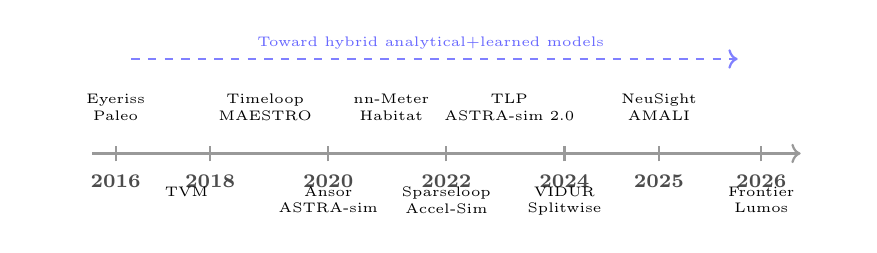
\begin{tikzpicture}[
    node distance=0.2cm,
    yearnode/.style={font=\scriptsize\bfseries, text=black!70},
    eventnode/.style={font=\tiny, text width=2cm, align=center},
    catnode/.style={font=\tiny, text=white, rounded corners=1pt, inner sep=2pt}
]
% Timeline base
\draw[thick, ->, black!40] (0,0) -- (9,0);
% Year markers
\foreach \x/\year in {0.3/2016, 1.5/2018, 3/2020, 4.5/2022, 6/2024, 7.2/2025, 8.5/2026} {
    \draw[thick, black!40] (\x,-0.1) -- (\x,0.1);
    \node[yearnode, below] at (\x,-0.15) {\year};
}
% Events
\node[eventnode, above] at (0.3,0.3) {Eyeriss\\Paleo};
\node[eventnode, below] at (1.2,-0.3) {TVM};
\node[eventnode, above] at (2.2,0.3) {Timeloop\\MAESTRO};
\node[eventnode, below] at (3,-0.3) {Ansor\\ASTRA-sim};
\node[eventnode, above] at (3.8,0.3) {nn-Meter\\Habitat};
\node[eventnode, below] at (4.5,-0.3) {Sparseloop\\Accel-Sim};
\node[eventnode, above] at (5.3,0.3) {TLP\\ASTRA-sim 2.0};
\node[eventnode, below] at (6,-0.3) {VIDUR\\Splitwise};
\node[eventnode, above] at (7.2,0.3) {NeuSight\\AMALI};
\node[eventnode, below] at (8.5,-0.3) {Frontier\\Lumos};
% Trend
\draw[thick, ->, blue!50, dashed] (0.5,1.2) -- (8.2,1.2);
\node[font=\tiny, text=blue!60, above] at (4.3,1.2) {Toward hybrid analytical+learned models};
\end{tikzpicture}%
}
\caption{Evolution of performance modeling tools (2016--2026). Early analytical frameworks gave way to systematic accelerator modeling and distributed training simulation. Recent work targets LLM-specific and hybrid approaches.}
\label{fig:timeline}
\end{figure}

% ==============================================================================
% SURVEY METHODOLOGY
% ==============================================================================
\section{Survey Methodology}
\label{sec:methodology}

We searched ACM Digital Library, IEEE Xplore, Semantic Scholar, and arXiv using terms related to ML performance modeling, with backward/forward citation tracking from seminal works.
Target venues include architecture (MICRO, ISCA, HPCA, ASPLOS), systems (MLSys, OSDI, SOSP, NSDI), and related (NeurIPS, MobiSys, DAC, ISPASS).
Papers must propose or evaluate a tool for predicting ML workload performance with quantitative evaluation; we exclude non-performance tasks and general-purpose workloads.
From 287 initial candidates, title/abstract screening yielded 118 papers; full-text review reduced the set to 53 that met all criteria, supplemented by 12 foundational works for context.
We cover 2016--2026 and classify each paper by \emph{methodology type} (analytical, simulation, trace-driven, ML-augmented, hybrid), \emph{target platform}, and \emph{abstraction level} (kernel, model, system).

\textbf{Related surveys and scope boundaries.}
Prior surveys address adjacent topics: Rakhshanfar and Zarandi~\cite{rakhshanfar2021survey} survey ML for processor DSE; Sze et al.~\cite{sze2017efficient} treat DNN hardware design; simulators such as GPGPU-Sim~\cite{gpgpusim2009}, gem5~\cite{binkert2011gem5}, and SST~\cite{sst2012} serve as validation targets; and MLPerf~\cite{mlperf_training2020,mlperf_inference2020} standardizes \emph{measurement} rather than \emph{prediction}.
Early accelerator modeling established foundational approaches: DianNao~\cite{diannao2014} introduced analytical dataflow modeling, Eyeriss~\cite{eyeriss2016} systematized row-stationary analysis, and Paleo~\cite{paleo2017} pioneered layer-wise estimation.
The closest prior work, Dudziak et al.~\cite{latencypredictorsnas2024}, compares edge device predictors for NAS; we broaden to the full landscape.

\textbf{Proprietary and vendor tools.}
NVIDIA's Nsight Compute~\cite{nsightcompute2019} and Nsight Systems are widely-used GPU profiling tools; Google's internal TPU models are undocumented.
We exclude these as they cannot be independently reproduced.

\textbf{Compiler cost models and capacity planning.}
Beyond TVM/Ansor/TLP, relevant models include Halide's autoscheduler~\cite{halide2013}, MLIR-based cost models~\cite{mlir2020}, and Triton's~\cite{triton2019} GPU kernel cost model.
Pollux~\cite{pollux2021} and Sia~\cite{sia2023} use performance models for cluster scheduling---a distinct use case sharing modeling techniques with our surveyed tools.
This survey differs from all prior work by spanning the full methodology spectrum across all major platforms with reproducibility evaluation.

% ==============================================================================
% BACKGROUND
% ==============================================================================
\section{Background}
\label{sec:background}

\subsection{ML Workload Characteristics}
\label{subsec:workload-characteristics}

ML workloads are computation graphs with statically known operator shapes amenable to analytical modeling. Frameworks such as PyTorch~\cite{pytorch2019} and TensorFlow~\cite{tensorflow2016} compile these graphs, though MoE and dynamic inference introduce input-dependent control flow.
Performance depends on dataflow/tiling, KV cache management~\cite{vllm2023}, and at scale, compute--memory--network interactions across data, tensor, pipeline, and expert parallelism~\cite{llama3scaling2025}.
LLM inference splits into compute-bound prefill and memory-bound decode phases~\cite{splitwise2024}, both modeled under batched serving~\cite{sarathi2024,orca2022}.
Training adds challenges: quadratic attention memory scaling, activation checkpointing, and mixed-precision effects~\cite{llama3scaling2025}.

\subsection{Modeling Methodologies}
\label{subsec:modeling-methodologies}

We classify approaches into five categories.
\textbf{Analytical models} express performance as closed-form functions (e.g., roofline~\cite{williams2009roofline}), offering microsecond evaluation but requiring per-architecture derivation.
\textbf{Cycle-accurate simulators} (GPGPU-Sim~\cite{gpgpusim2009}, Accel-Sim~\cite{accelsim2020}) achieve high fidelity at $1000$--$10000\times$ slowdown, serving as validation oracles.
\textbf{Trace-driven simulators} (ASTRA-sim~\cite{astrasim2023}, VIDUR~\cite{vidur2024}) trade fidelity for orders-of-magnitude speedup.
\textbf{ML-augmented approaches} learn from profiling data (nn-Meter~\cite{nnmeter2021}) but may not generalize beyond training distributions.
\textbf{Hybrid approaches} combine analytical structure with learned components (NeuSight~\cite{neusight2025}, Habitat~\cite{habitat2021}).
Accuracy metrics---MAPE, RMSE, rank correlation---vary across the literature, limiting direct comparison (Section~\ref{sec:eval-results}); ground-truth relies on hardware counters (PAPI~\cite{papi2000}, LIKWID~\cite{likwid2010}) or vendor profilers~\cite{nsightcompute2019}.

% ==============================================================================
% TAXONOMY
% ==============================================================================
\section{Taxonomy}
\label{sec:taxonomy}

We organize the literature along three dimensions: \emph{methodology type} (primary axis), \emph{target platform}, and \emph{abstraction level}, additionally identifying a temporal validation lag: pre-2023 tools validated on CNNs, while post-2023 tools target transformers and LLMs.
Table~\ref{tab:taxonomy-matrix} provides a unified coverage matrix with trade-off profiles; the dominant pairings are analytical models for accelerators, cycle-accurate simulation for GPUs/CPUs, trace-driven simulation for distributed systems, and ML-augmented approaches for edge devices.

\begin{table*}[t]
\centering
\caption{Methodology taxonomy: coverage matrix and trade-off profile. \textbf{0} = research gap.}
\label{tab:taxonomy-matrix}
\small
\begin{tabular}{l|ccccc|cccc}
\toprule
 & \textbf{DNN} & & \textbf{Distrib.} & \textbf{Edge/} & & \textbf{Eval.} & \textbf{Data} & & \textbf{Failure} \\
\textbf{Methodology} & \textbf{Accel.} & \textbf{GPU} & \textbf{Systems} & \textbf{Mobile} & \textbf{CPU} & \textbf{Speed} & \textbf{Req.} & \textbf{Interp.} & \textbf{Mode} \\
\midrule
Analytical       & 3 & 3 & 2 & \textbf{0} & \textbf{0} & $\mu$s & None & High & Dynamic effects \\
Cycle-Accurate   & 1 & 2 & \textbf{0} & \textbf{0} & 1 & Hours & Binary & High & Scale \\
Trace-Driven     & \textbf{0} & \textbf{0} & 7 & \textbf{0} & \textbf{0} & Min. & Traces & Med. & Trace fidelity \\
ML-Augmented     & \textbf{0} & 3 & \textbf{0} & 3 & 1 & ms & Profiling & Low & Distrib.\ shift \\
Hybrid           & 1 & 2 & \textbf{0} & \textbf{0} & 1 & ms & Mixed & Med. & Training domain \\
\bottomrule
\end{tabular}
\end{table*}

Three structural gaps emerge: (1)~trace-driven execution replay is used exclusively for distributed systems; (2)~edge devices lack hybrid alternatives; (3)~no ML-augmented tool targets distributed systems.
Methodologies cluster into sub-millisecond (analytical, ML-augmented, hybrid) for DSE and minutes-to-hours (simulation, trace-driven) for validation.
Figure~\ref{fig:tool-architecture} illustrates how methodology types compose.

\begin{figure}[t]
\centering
\resizebox{\columnwidth}{!}{%
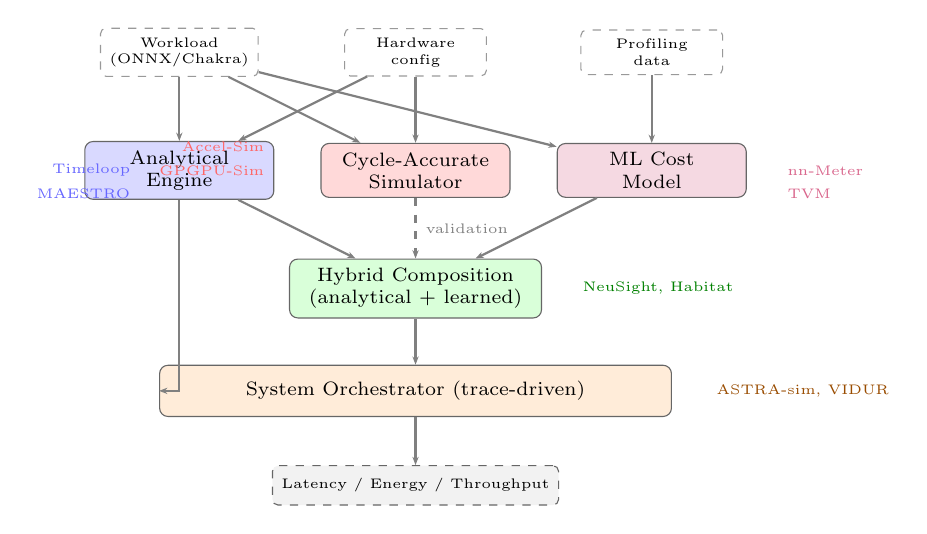
\begin{tikzpicture}[
    comp/.style={draw=black!60, rounded corners=3pt, minimum width=2.4cm, minimum height=0.65cm, align=center, font=\scriptsize},
    input/.style={draw=black!40, dashed, rounded corners=2pt, minimum width=1.8cm, minimum height=0.5cm, align=center, font=\tiny},
    arr/.style={-{Stealth[length=3pt]}, thick, black!50},
    lbl/.style={font=\tiny, text=black!50},
]

% Input layer
\node[input] (wl) at (0,4) {Workload\\(ONNX/Chakra)};
\node[input] (hw) at (3,4) {Hardware\\config};
\node[input] (prof) at (6,4) {Profiling\\data};

% Methodology layer
\node[comp, fill=blue!15] (analytical) at (0,2.5) {Analytical\\Engine};
\node[comp, fill=red!15] (simulator) at (3,2.5) {Cycle-Accurate\\Simulator};
\node[comp, fill=purple!15] (mlmodel) at (6,2.5) {ML Cost\\Model};

% Hybrid composition
\node[comp, fill=green!15, minimum width=3.2cm] (hybrid) at (3,1) {Hybrid Composition\\(analytical + learned)};

% System orchestration
\node[comp, fill=orange!15, minimum width=6.5cm] (system) at (3,-0.3) {System Orchestrator (trace-driven)};

% Output
\node[input, draw=black!60, fill=gray!10] (output) at (3,-1.5) {Latency / Energy / Throughput};

% Arrows - inputs to methods
\draw[arr] (wl) -- (analytical);
\draw[arr] (hw) -- (analytical);
\draw[arr] (hw) -- (simulator);
\draw[arr] (wl) -- (simulator);
\draw[arr] (prof) -- (mlmodel);
\draw[arr] (wl) -- (mlmodel);

% Arrows - methods to hybrid
\draw[arr] (analytical) -- (hybrid);
\draw[arr] (mlmodel) -- (hybrid);
\draw[arr, dashed, gray] (simulator) -- node[lbl, right] {validation} (hybrid);

% Arrows - to system
\draw[arr] (hybrid) -- (system);
\draw[arr] (analytical) |- (system);

% Arrows - output
\draw[arr] (system) -- (output);

% Example tools
\node[font=\tiny, text=blue!60, anchor=east] at (-0.5,2.5) {Timeloop};
\node[font=\tiny, text=blue!60, anchor=east] at (-0.5,2.2) {MAESTRO};
\node[font=\tiny, text=red!60, anchor=east] at (1.2,2.8) {Accel-Sim};
\node[font=\tiny, text=red!60, anchor=east] at (1.2,2.5) {GPGPU-Sim};
\node[font=\tiny, text=purple!60, anchor=west] at (7.6,2.5) {nn-Meter};
\node[font=\tiny, text=purple!60, anchor=west] at (7.6,2.2) {TVM};
\node[font=\tiny, text=green!50!black, anchor=west] at (5,1) {NeuSight, Habitat};
\node[font=\tiny, text=orange!60!black, anchor=west] at (6.7,-0.3) {ASTRA-sim, VIDUR};

\end{tikzpicture}%
}
\caption{Unified architecture showing how tool methodologies compose.}
\label{fig:tool-architecture}
\end{figure}

\subsection{Methodology--Platform Pairings}
\label{subsec:by-methodology}

Platform constrains methodology (Table~\ref{tab:taxonomy-matrix}): \textbf{accelerators} use analytical models~\cite{timeloop2019,maestro2019}; \textbf{GPUs} span all five types; \textbf{distributed systems} require trace-driven simulation~\cite{astrasim2023,vidur2024}; \textbf{edge devices} rely on ML-augmented approaches~\cite{nnmeter2021,litepred2024}; \textbf{CPUs}~\cite{concorde2025,granite2022} are least studied.
Abstraction level determines composition errors (Figure~\ref{fig:abstraction-levels}): kernel-level 2--3\%, model-level 5--12\%, system-level 5--15\%, with errors propagating through the chain.

\begin{figure}[t]
\centering
\resizebox{\columnwidth}{!}{%
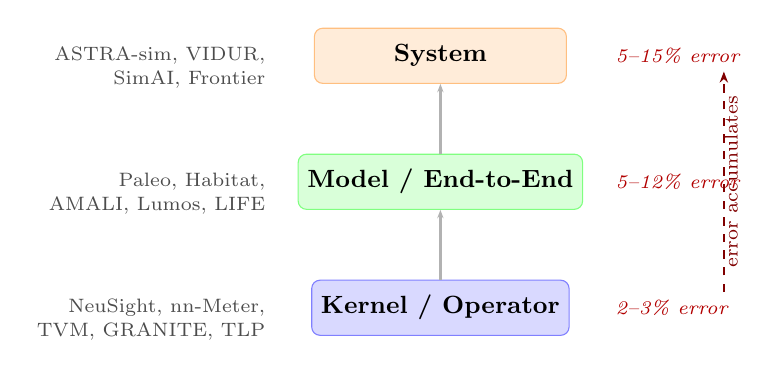
\begin{tikzpicture}[
  level/.style={draw, rounded corners=3pt, minimum width=3.2cm, minimum height=0.7cm, align=center, font=\small\bfseries},
  tool/.style={font=\scriptsize, text=black!70},
  err/.style={font=\scriptsize\itshape, text=red!70!black},
  arrow/.style={-{Stealth[length=3pt]}, thick, gray!60},
  compos/.style={-{Stealth[length=4pt]}, thick, red!50!black, dashed},
]

% Levels (bottom to top)
\node[level, fill=blue!15, draw=blue!50] (kernel) at (0,0) {Kernel / Operator};
\node[level, fill=green!15, draw=green!50] (model) at (0,1.6) {Model / End-to-End};
\node[level, fill=orange!15, draw=orange!50] (system) at (0,3.2) {System};

% Composition arrows between levels
\draw[arrow] (kernel) -- (model);
\draw[arrow] (model) -- (system);

% Tool names (left side)
\node[tool, anchor=east] at (-2.1,0) {NeuSight, nn-Meter,};
\node[tool, anchor=east] at (-2.1,-0.3) {TVM, GRANITE, TLP};
\node[tool, anchor=east] at (-2.1,1.6) {Paleo, Habitat,};
\node[tool, anchor=east] at (-2.1,1.3) {AMALI, Lumos, LIFE};
\node[tool, anchor=east] at (-2.1,3.2) {ASTRA-sim, VIDUR,};
\node[tool, anchor=east] at (-2.1,2.9) {SimAI, Frontier};

% Error ranges (right side)
\node[err, anchor=west] at (2.1,0) {2--3\% error};
\node[err, anchor=west] at (2.1,1.6) {5--12\% error};
\node[err, anchor=west] at (2.1,3.2) {5--15\% error};

% Composition problem annotation
\draw[compos] (3.6,0.2) -- (3.6,3.0);
\node[font=\scriptsize, text=red!50!black, rotate=90, anchor=south] at (3.9,1.6) {error accumulates};

\end{tikzpicture}%
}
\caption{Abstraction level hierarchy. Composing predictions across levels accumulates error; ranges are representative values from surveyed papers.}
\label{fig:abstraction-levels}
\end{figure}

\subsection{Workload Coverage and Validation Gaps}
\label{subsec:workload-coverage}

Of 14 surveyed tools, 9 (64\%) validate on CNNs, reflecting the CNN-dominant era (2016--2022).
The lag is closing---post-2023 tools validate exclusively on transformers/LLMs---but \textbf{no tool validates on diffusion models or dynamic inference}~\cite{dynamicreasoning2026}, only Frontier~\cite{frontier2025} validates MoE, and no tool offers validated transformer prediction across the full kernel-to-system stack.

% ==============================================================================
% SURVEY OF APPROACHES
% ==============================================================================
\section{Survey of Approaches}
\label{sec:survey}

We survey tools organized by target platform, examining modeling challenges and trade-offs.
Table~\ref{tab:survey-summary} provides a comprehensive comparison.

\begin{table*}[t]
\centering
\caption{Surveyed tools by target platform. A=Analytical, S=Simulation, T=Trace-driven, M=ML-augmented, H=Hybrid. $^*$Surrogate-vs-simulator fidelity. $^\dagger$Unverifiable. $^\ddagger$No hardware baseline.}
\label{tab:survey-summary}
\small
\begin{tabular}{lllllll}
\toprule
\textbf{Tool} & \textbf{Platform} & \textbf{Method} & \textbf{Target} & \textbf{Accuracy} & \textbf{Speed} & \textbf{Key Capability} \\
\midrule
\multicolumn{7}{l}{\textit{DNN Accelerator Modeling}} \\
Timeloop~\cite{timeloop2019} & NPU & A & Latency/Energy & 5--10\% & $\mu$s & Loop-nest DSE \\
MAESTRO~\cite{maestro2019} & NPU & A & Latency/Energy & 5--15\% & $\mu$s & Data-centric directives \\
Sparseloop~\cite{sparseloop2022} & NPU & A & Sparse tensors & 5--10\% & $\mu$s & Compression modeling \\
PyTorchSim~\cite{pytorchsim2025} & NPU & S & Cycle-accurate & N/A$^\ddagger$ & Hours & PyTorch 2 integration \\
ArchGym~\cite{archgym2023} & Multi & H & Multi-objective & 0.61\%$^*$ & ms & ML-aided DSE \\
\midrule
\multicolumn{7}{l}{\textit{GPU Performance Modeling}} \\
Accel-Sim~\cite{accelsim2020} & GPU & S & Cycle-accurate & 10--20\% & Hours & SASS trace-driven \\
GPGPU-Sim~\cite{gpgpusim2009} & GPU & S & Cycle-accurate & 10--20\% & Hours & CUDA workloads \\
AMALI~\cite{amali2025} & GPU & A & LLM inference & 23.6\% & ms & Memory hierarchy \\
NeuSight~\cite{neusight2025} & GPU & H & Kernel/E2E latency & 2.3\% & ms & Tile-based prediction \\
Habitat~\cite{habitat2021} & GPU & H & Training time & 11.8\% & Per-kernel & Wave scaling \\
\midrule
\multicolumn{7}{l}{\textit{Distributed Training and LLM Serving}} \\
ASTRA-sim~\cite{astrasim2023} & Distributed & T & Training time & 5--15\% & Minutes & Collective modeling \\
SimAI~\cite{simai2025} & Distributed & T & Training time & 1.9\% & Minutes & Full-stack simulation \\
Lumos~\cite{lumos2025} & Distributed & T & LLM training & 3.3\% & Minutes & H100 training \\
VIDUR~\cite{vidur2024} & GPU cluster & T & LLM serving & $<$5\% & Seconds & Prefill/decode phases \\
Frontier~\cite{frontier2025} & Distributed & T & MoE inference & --- & Minutes & Stage-centric sim. \\
TrioSim~\cite{triosim2025} & Multi-GPU & T & DNN training & N/A$^\ddagger$ & Minutes & Lightweight multi-GPU \\
\midrule
\multicolumn{7}{l}{\textit{Edge Device Modeling}} \\
nn-Meter~\cite{nnmeter2021} & Edge & M & Latency & $<$1\%$^\dagger$ & ms & Kernel detection \\
LitePred~\cite{litepred2024} & Edge & M & Latency & 0.7\% & ms & 85-platform transfer \\
HELP~\cite{help2021} & Multi & M & Latency & 1.9\% & ms & 10-sample adaptation \\
\midrule
\multicolumn{7}{l}{\textit{Compiler Cost Models}} \\
TVM~\cite{tvm2018} & GPU & M & Schedule perf. & $\sim$15\% & ms & Autotuning guidance \\
Ansor~\cite{ansor2020} & GPU & M & Schedule perf. & $\sim$15\% & ms & Program sampling \\
TLP~\cite{tlp2023} & GPU & M & Tensor program & $<$10\% & ms & Transformer cost model \\
\bottomrule
\end{tabular}
\end{table*}

\subsection{DNN Accelerator Modeling}
\label{subsec:accelerator-modeling}

The analytical tractability of DNN accelerator modeling stems from computational regularity~\cite{sze2017efficient}, building on DianNao~\cite{diannao2014} and Eyeriss~\cite{eyeriss2016}.
Timeloop~\cite{timeloop2019} enumerates mappings of loop nests to a spatial-temporal hardware hierarchy, finding optimal dataflow in microseconds (5--10\% error, $2000\times$ speedup).
MAESTRO~\cite{maestro2019} uses a compact ``data-centric'' representation, trading completeness for simplicity.
Sparseloop~\cite{sparseloop2022} extends to sparse tensors (CSR, bitmap); SCALE-Sim~\cite{scalesim2019} provides cycle-accurate systolic array validation.
PyTorchSim~\cite{pytorchsim2025} and ArchGym~\cite{archgym2023} (0.61\% RMSE vs.\ simulator) represent newer approaches.
This is the most mature subdomain; emerging PIM tools~\cite{upimulator2024,attacc2024,neupims2024,paise2025} also lack hardware validation.

\subsection{GPU Performance Modeling}
\label{subsec:gpu-modeling}

GPGPU-Sim~\cite{gpgpusim2009} and Accel-Sim~\cite{accelsim2020} achieve 0.90--0.97 IPC correlation at $1000$--$10000\times$ slowdown, integrating with memory models (DRAMSim3~\cite{dramsim3_2020}, Ramulator~2.0~\cite{ramulator2_2023}); reverse-engineering~\cite{dissectinggpu2025} improved Accel-Sim to 13.98\% MAPE.
NeuSight~\cite{neusight2025} achieves 2.3\% MAPE by decomposing kernels into \emph{tiles} matching CUDA thread blocks, succeeding because each SM's execution depends on locally measurable arithmetic intensity, shared memory, and register pressure.
AMALI~\cite{amali2025} averages data movement over entire kernels (23.6\% MAPE); the roofline model~\cite{williams2009roofline,rooflinellm2024} provides upper bounds.
Habitat~\cite{habitat2021} achieves 11.8\% cross-GPU transfer via wave scaling.
VIDUR~\cite{vidur2024} simulates LLM serving at $<$5\% error; TVM~\cite{tvm2018}/Ansor~\cite{ansor2020} ($\sim$15\%), TLP~\cite{tlp2023} ($<$10\%), and recent tools~\cite{life2025,hermes2025,omniwise2025,swizzleperf2025,synperf2025} target inference and autotuning~\cite{tenset2021}.

\subsection{Distributed Training and LLM Serving}
\label{subsec:distributed-modeling}

Distributed systems require modeling communication, synchronization, and parallelism~\cite{megatronlm2020,gpipe2019,zero2020}.
The speed--fidelity hierarchy reflects granularity: VIDUR models serving at the \emph{request level}; ASTRA-sim~\cite{astrasim2023} replays Chakra traces~\cite{chakra2023} at the \emph{collective level} (5--15\%); SimAI~\cite{simai2025} models \emph{NCCL-level} chunk reductions (1.9\%), capturing non-linear congestion invisible to per-collective models.
Echo~\cite{echo2024} scales to 10K+ devices; Lumos~\cite{lumos2025} achieves 3.3\% on H100s; PRISM~\cite{prism2025} provides prediction intervals; Paleo~\cite{paleo2017}, MAD Max~\cite{madmax2024}, and Sailor~\cite{sailor2025} provide analytical estimation.
For inference serving, DistServe~\cite{distserve2024}, Frontier~\cite{frontier2025} (MoE), POD-Attention~\cite{podattention2025}, AQUA~\cite{aqua2025}, and ThrottLL'eM~\cite{throttllem2025} address scheduling, disaggregation, and power; speculative decoding~\cite{medusa2024} creates a moving target.

\subsection{Edge Device Modeling}
\label{subsec:edge-modeling}

nn-Meter~\cite{nnmeter2021} claims $<$1\% MAPE but is unverifiable due to dependency failures (Section~\ref{sec:eval-results}); LitePred~\cite{litepred2024} achieves 0.7\% across 85 platforms; HELP~\cite{help2021} reaches 1.9\% with 10-sample meta-learning.
ESM~\cite{esm2025} finds well-tuned random forests match deep learning surrogates, and transfer learning provides 22.5\% improvement~\cite{latencypredictorsnas2024}---suggesting data quality matters more than model sophistication.

% ==============================================================================
% EVALUATION FRAMEWORK
% ==============================================================================
\section{Evaluation Methodology}
\label{sec:eval-framework}

Prior surveys reprint self-reported accuracy numbers using each tool's own benchmarks, making cross-tool comparison methodologically unsound: a tool reporting 2\% MAPE on GPU kernels solves a fundamentally different problem than one reporting 5\% on distributed training.
We take a different approach: we define an \textbf{LLM-focused benchmark suite} representing concrete user needs for modern LLM training and inference, then evaluate each tool's capability against this suite through \textbf{accuracy-centered independent experiments}.

\textbf{Evaluation principle.}
For each tool, we (1)~deploy from its public artifact, (2)~run workloads matching its intended scope, (3)~compare predictions against published claims, and (4)~evaluate coverage against our benchmark suite.
Where absolute verification requires hardware we lack (e.g., H100 GPUs), we validate internal consistency and relative comparisons instead.

\subsection{LLM Benchmark Suite}
\label{subsec:benchmark-suite}

We define 28 benchmark scenarios across 8 categories representing the workloads that LLM practitioners need performance predictions for (Table~\ref{tab:benchmark-suite}).
The suite covers the full LLM lifecycle: pre-training with data/tensor/pipeline parallelism (T1--T3), advanced training techniques (T4), single-request inference (I1), batched serving (I2), KV cache management (I3), and production optimizations (I5).

\begin{table}[t]
\centering
\caption{LLM benchmark suite: 28 scenarios across training (T1--T4) and inference (I1--I5). Each represents a concrete user need for performance prediction.}
\label{tab:benchmark-suite}
\small
\begin{tabular}{lp{3.5cm}r}
\toprule
\textbf{Cat.} & \textbf{Description} & \textbf{\#} \\
\midrule
T1 & Data-parallel pre-training & 3 \\
T2 & Tensor-parallel pre-training & 2 \\
T3 & Pipeline-parallel pre-training & 2 \\
T4 & Advanced (FP8, LoRA, SP, MoE) & 4 \\
\midrule
I1 & Single-request inference & 3 \\
I2 & Batched serving (vLLM, Sarathi) & 3 \\
I3 & KV cache management & 2 \\
I4 & Multi-model serving & 1 \\
I5 & Production (spec.\ decode, quant.) & 4 \\
\midrule
& \textbf{Total} & \textbf{28} \\
\bottomrule
\end{tabular}
\end{table}

\textbf{Design principles.}
Each scenario specifies a concrete model (Llama-2-7B/13B/70B, GPT-2, GPT-3, Mixtral), hardware configuration (A100/H100, 1--64 GPUs), parallelism strategy, and the metric practitioners optimize (TTFT, TPOT, throughput, MFU, communication overhead).
Training scenarios span from single-node data parallelism (T1.1: GPT-2 on 8$\times$A100) to large-scale hybrid parallelism (T3.2: GPT-3 175B on 64$\times$H100 with PP8+TP8).
Inference scenarios range from single-request latency (I1.1) to production optimizations like speculative decoding (I5.1) and disaggregated serving (I5.4).

\textbf{Coverage criterion.}
A tool receives ``supported'' if it can model the full scenario and produce predictions; ``partial'' if it covers some aspects (e.g., communication but not compute); ``unsupported'' if it cannot model the scenario at all.

\subsection{Tool Selection}
\label{subsec:tool-selection}

From 22 tools, we select 5 using three criteria: (1)~\emph{methodology coverage}---one per type; (2)~\emph{artifact availability}---open-source with build instructions; (3)~\emph{scope diversity}---different hardware and workload types.
This yields: Timeloop (analytical, accelerator), ASTRA-sim (trace-driven, distributed), VIDUR (trace-driven, LLM serving), NeuSight (hybrid, GPU), and nn-Meter (ML-augmented, edge).
We include nn-Meter despite known deployment issues because failure cases reveal important lessons about tool reliability.

\subsection{Experimental Design}
\label{subsec:experimental-design}

Experiments match each tool's intended scope:
\textbf{NeuSight:} 146 configurations across 12 GPU types (NVIDIA V100, H100, A100-80G, A100-40G, L4, T4, P100, P4; AMD MI100, MI210, MI250).
\textbf{ASTRA-sim:} 4 collectives at 8~NPUs on HGX-H100, plus ResNet-50 at 2/4/8 GPUs.
\textbf{VIDUR:} Llama-2-7B on simulated A100 under vLLM and Sarathi schedulers.
\textbf{Timeloop:} ResNet-50 Conv1 on Eyeriss-like architecture.
\textbf{nn-Meter:} Attempted deployment across 4 edge device targets.
All experiments run on Apple M2 Ultra (192\,GB RAM, Docker where available).
Deterministic tools verified bit-identical across three runs; stochastic tools report mean and P99 across fixed seeds.
Scripts and data are provided as supplementary material.

\subsection{Limitations}
\label{subsec:eval-limitations}

Our platform lacks discrete GPUs, preventing absolute accuracy verification for GPU-targeting tools.
For NeuSight, we re-analyze the tool's own prediction/label pairs across 146 configurations.
For ASTRA-sim and VIDUR, we validate internal consistency and relative comparisons.
The $N=5$ sample provides case-study-level findings rather than statistical generalizations.

% ==============================================================================
% EVALUATION RESULTS
% ==============================================================================
\section{Evaluation Results}
\label{sec:eval-results}

Table~\ref{tab:accuracy-comparison} summarizes accuracy findings; Table~\ref{tab:feature-matrix} presents the feature availability matrix.

\begin{table}[t]
\centering
\caption{Accuracy comparison: published claims vs.\ our independent verification.}
\label{tab:accuracy-comparison}
\small
\begin{tabular}{lp{1.5cm}p{1.5cm}p{2.2cm}}
\toprule
\textbf{Tool} & \textbf{Published} & \textbf{Our Result} & \textbf{Verdict} \\
\midrule
NeuSight & 2.3\% MAPE & 5.87--27.1\% & Overstated 2--4$\times$ \\
ASTRA-sim & 9.69\% geo. & Trends valid & Plausible, unverified \\
VIDUR & $<$5\% err. & Ranking valid & Plausible, unverified \\
Timeloop & $<$10\% RTL & Structure valid & Consistent w/ Eyeriss \\
nn-Meter & $<$1\% MAPE & \textbf{No output} & Complete failure \\
\bottomrule
\end{tabular}
\end{table}

\begin{table*}[t]
\centering
\caption{Feature availability matrix. ``---'' = no capability. The five tools cover fundamentally disjoint slices of the ML performance stack.}
\label{tab:feature-matrix}
\small
\begin{tabular}{lccccc}
\toprule
\textbf{Feature} & \textbf{NeuSight} & \textbf{ASTRA-sim} & \textbf{VIDUR} & \textbf{Timeloop} & \textbf{nn-Meter} \\
\midrule
\multicolumn{6}{l}{\emph{Workload Types}} \\
CNN training/inference & Full model & Comm only & --- & Single-layer energy & Inf.\ latency only \\
Transformer training & Single-GPU time & Comm patterns & --- & --- & --- \\
LLM inference serving & --- & --- & Full (TTFT/TPOT) & --- & --- \\
Accelerator design space & --- & --- & --- & Full (dataflow) & --- \\
Edge inference & --- & --- & --- & --- & Full (broken) \\
\midrule
\multicolumn{6}{l}{\emph{Hardware Targets}} \\
NVIDIA datacenter GPU & 7 types & Comm only & A100/H100 & --- & --- \\
AMD GPU & MI100/MI210/MI250 & --- & --- & --- & --- \\
Custom accelerator & --- & --- & --- & Eyeriss, systolic & --- \\
Edge device & --- & --- & --- & --- & ARM, Adreno, Myriad \\
Multi-GPU cluster & DP/PP/TP (limited) & 2--16 GPUs & --- & --- & --- \\
\midrule
\multicolumn{6}{l}{\emph{Prediction Granularity}} \\
Kernel/layer level & Per-layer (tiles) & --- & --- & Per-layer energy & Per-kernel models \\
Model level & Sum of layers & Comm only & Full iteration & --- & Sum of kernels \\
System level & --- & Comm + compute & Request scheduling & --- & --- \\
\midrule
\multicolumn{6}{l}{\emph{Metrics}} \\
Latency & GPU kernel (ms) & Comm cycles & E2E, TTFT, TPOT & Cycle count & Inf.\ latency (ms) \\
Energy & --- & --- & --- & Full breakdown & --- \\
Throughput & --- & --- & Tokens/s, req/s & --- & --- \\
Memory & --- & --- & KV cache & Buffer sizes & --- \\
\bottomrule
\end{tabular}
\end{table*}

\subsection{NeuSight: GPU Kernel Accuracy}
\label{subsec:neusight-results}

NeuSight claims 2.3\% overall MAPE for GPU kernel latency prediction~\cite{neusight2025}.
We independently re-analyzed 146 model configurations across 12 GPU types using the tool's own prediction/label pairs (Table~\ref{tab:neusight-accuracy}).

\begin{table}[t]
\centering
\caption{NeuSight accuracy: published claims vs.\ our verification across 12 GPU types. $N$: number of model configurations tested. Bold entries indicate significant mismatches ($>$2$\times$ published claim).}
\label{tab:neusight-accuracy}
\small
\begin{tabular}{llrrl}
\toprule
\textbf{Device} & \textbf{Mode} & \textbf{Claimed} & \textbf{Ours} & \textbf{Verdict} \\
\midrule
V100 & Inference & 5.2\% & 5.87\% & Match \\
V100 & Training & 7.4\% & 8.91\% & Close \\
H100 & Inference & 2.3\% & \textbf{8.74\%} & Mismatch \\
H100 & Training & 4.1\% & 6.60\% & Close \\
A100-80G & Training & 5.8\% & 7.59\% & Close \\
A100-40G & Inference & --- & 8.63\% & --- \\
L4 & Inference & 3.8\% & \textbf{14.08\%} & Mismatch \\
T4 & Inference & 6.1\% & \textbf{18.51\%} & Mismatch \\
P4 & Inference & --- & \textbf{27.10\%} & --- \\
MI100 & Inference & --- & 10.80\% & --- \\
MI210 & Inference & --- & 8.40\% & --- \\
MI250 & Inference & --- & 7.65\% & --- \\
\bottomrule
\end{tabular}
\end{table}

\textbf{Key finding: accuracy degrades outside the training distribution.}
NeuSight achieves its best accuracy on V100 (5.87\%), the GPU most represented in training data.
On newer GPUs (H100: 8.74\% vs.\ claimed 2.3\%, a $3.8\times$ gap) and older GPUs (T4: 18.51\%, P4: 27.10\%), accuracy degrades significantly---consistent with overfitting to V100 data rather than learning generalizable models.
The worst-case max APE reaches 65.30\% on P4.
Models tested include BERT-Large, GPT-2-Large, GPT-3, OPT-13B, and SwitchXL4.

\subsection{ASTRA-sim: Distributed Training Communication}
\label{subsec:astrasim-results}

ASTRA-sim reports 9.69\% geomean error at 8-GPU HGX-H100 for Ring All-Reduce~\cite{astrasim2020}.
We ran collective microbenchmarks and ResNet-50 data-parallel training scaling (Table~\ref{tab:astrasim-results}).

\begin{table}[t]
\centering
\caption{ASTRA-sim results on HGX-H100 configuration from our experiments. Top: collectives (8 NPUs, 1\,MB). Bottom: ResNet-50 scaling.}
\label{tab:astrasim-results}
\small
\begin{tabular}{lrr}
\toprule
\multicolumn{3}{l}{\textbf{Collective Microbenchmarks (8 NPUs, 1\,MB)}} \\
\midrule
\textbf{Collective} & \textbf{Cycles} & \textbf{Ratio vs.\ AR} \\
\midrule
All-Reduce & 57,426 & 1.000 \\
All-Gather & 44,058 & 0.767 \\
Reduce-Scatter & 28,950 & 0.504 \\
All-to-All & 114,000 & 1.985 \\
\midrule
\multicolumn{3}{l}{\textbf{ResNet-50 Data-Parallel Training}} \\
\midrule
\textbf{GPUs} & \textbf{Comm Cycles} & \textbf{Comm Overhead} \\
\midrule
2 & 574,289 & 0.05\% \\
4 & 1,454,270 & 0.13\% \\
8 & 3,307,886 & 0.30\% \\
\bottomrule
\end{tabular}
\end{table}

\textbf{Internal consistency is strong.}
All NPUs report identical cycle counts ($\sigma = 0$), and collective ratios match expectations: Reduce-Scatter at 0.504$\times$ All-Reduce (half-data operation), All-to-All at 1.985$\times$ (personalized exchange).
Communication scales as expected from 4 to 8 GPUs ($2.27\times$).

\textbf{Absolute accuracy is unverifiable} without HGX-H100 hardware.
ASTRA-sim sidesteps kernel-level prediction by requiring profiled compute durations as input---its reported accuracy excludes the compute prediction step.

\subsection{VIDUR: LLM Inference Serving}
\label{subsec:vidur-results}

VIDUR reports $<$5\% error vs.\ real serving traces~\cite{vidur2024}.
We simulated Llama-2-7B on a simulated A100 under two scheduler configurations (Table~\ref{tab:vidur-results}).

\begin{table}[t]
\centering
\caption{VIDUR simulation: Llama-2-7B on simulated A100 (Poisson arrivals, QPS~2.0, seed=42). All metrics from our experiments.}
\label{tab:vidur-results}
\small
\begin{tabular}{lcc}
\toprule
\textbf{Metric} & \textbf{vLLM} & \textbf{Sarathi} \\
\midrule
Requests & 200 & 50 \\
Avg E2E latency (s) & 0.177 & 0.158 \\
P99 E2E latency (s) & 0.314 & 0.262 \\
Avg TTFT (s) & 0.027 & 0.025 \\
Avg TPOT (s) & 0.0093 & 0.0090 \\
Preempted requests & 53 & 0 \\
\bottomrule
\end{tabular}
\end{table}

\textbf{Scheduler ranking is correct.}
Sarathi~\cite{sarathi2024} achieves 12.2\% lower E2E latency and eliminates preemption (0 vs.\ 53 requests), consistent with its chunked-prefill design.
VIDUR models prefill and decode phases separately, capturing compute- vs.\ memory-bound regimes.
Absolute values require A100 hardware for verification.

\subsection{Timeloop: Accelerator Energy/Performance}
\label{subsec:timeloop-results}

Timeloop reports accuracy within 10\% of RTL simulation for energy, validated against Eyeriss silicon~\cite{timeloop2019}.
We ran ResNet-50 Conv1 on an Eyeriss-like architecture:

\begin{itemize}
    \item Total energy: 649.08~\textmu{}J (5,500~fJ/MAC) with DRAM dominating (61.8\%), followed by weights SPAD (18.4\%) and MAC (3.8\%)
    \item Estimated latency: 5.854~ms at $\sim$60\% utilization (168 PEs, 702,464 ideal cycles)
    \item Outputs are deterministic and bit-identical across three runs
\end{itemize}

The energy breakdown structure matches published Eyeriss data~\cite{eyeriss2016}: DRAM dominance and small MAC energy fraction are characteristic of data-movement-dominated architectures.
Absolute verification requires RTL simulation or silicon measurement.

\subsection{nn-Meter: Complete Failure}
\label{subsec:nnmeter-results}

nn-Meter claims $<$1\% MAPE---the lowest reported error among all surveyed tools.
After four deployment attempts ($>$4 hours), we obtained \textbf{zero predictions}: pre-trained models serialized with scikit-learn 0.23.1 (2020) cannot be deserialized with current versions.
Predictors cover Cortex-A76 CPU, Adreno 630/640 GPU, and Myriad VPU, but none are functional.
\textbf{The tool claiming the best accuracy is the only tool that produces no output}---pickle serialization without version pinning created an expiration date, rendering the tool unusable within two years.

\subsection{Benchmark Suite Coverage}
\label{subsec:benchmark-coverage}

Table~\ref{tab:benchmark-coverage} evaluates each tool against our 28-scenario LLM benchmark suite.
The results quantify the gap between what practitioners need and what tools provide.

\begin{table}[t]
\centering
\caption{Tool coverage of LLM benchmark suite (28 scenarios). S=Supported, P=Partial, U=Unsupported. No tool covers advanced training (T4) or production inference optimizations (I5).}
\label{tab:benchmark-coverage}
\small
\begin{tabular}{lcccccc}
\toprule
\textbf{Category} & \textbf{\#} & \textbf{Neu.} & \textbf{AST.} & \textbf{VID.} & \textbf{TL} & \textbf{nn-M} \\
\midrule
T1: Data parallel  & 3 & 2P & 3S & --- & --- & --- \\
T2: Tensor parallel & 2 & 2P & 2S & --- & --- & --- \\
T3: Pipeline parallel & 2 & 2P & 2S & --- & --- & --- \\
T4: Advanced train. & 4 & --- & 2P & --- & --- & --- \\
\midrule
I1: Single request & 3 & 2S,1P & --- & 2S,1P & --- & --- \\
I2: Batched serving & 3 & --- & --- & 3S & --- & --- \\
I3: KV cache & 2 & --- & --- & 1S,1P & --- & --- \\
I4: Multi-model & 1 & --- & --- & --- & --- & --- \\
I5: Production opt. & 4 & --- & --- & --- & --- & --- \\
\midrule
\textbf{Supported} & & 5 & 7 & 6 & 0 & 0 \\
\textbf{Partial} & & 3 & 2 & 2 & 0 & 0 \\
\textbf{Coverage} & & 18\% & 25\% & 21\% & 0\% & 0\% \\
\bottomrule
\end{tabular}
\end{table}

\textbf{Half of LLM workloads have zero tool coverage.}
Of 28 scenarios, 14 (50\%) are not addressable by any evaluated tool.
The entirely uncovered scenarios include FP8 mixed-precision training (T4.1), LoRA fine-tuning (T4.2), speculative decoding (I5.1), prefix caching (I5.2), INT4 quantized inference (I5.3), disaggregated serving (I5.4), and multi-model co-location (I4.1).
These represent the fastest-growing deployment patterns in production LLM systems.

\textbf{Tools cover disjoint slices.}
ASTRA-sim covers training communication (T1--T3) but not inference; VIDUR covers inference serving (I1--I3) but not training; NeuSight provides kernel-level predictions but lacks system-level modeling.
Only 3 scenarios (I1.1, I1.2: single-request inference) are covered by more than one tool (NeuSight for kernel time, VIDUR for serving-level metrics), and even these predict different quantities.

\textbf{Modern techniques are the largest gap.}
Categories T4 (advanced training) and I5 (production optimizations) have near-zero coverage despite representing the techniques practitioners most need predictions for when making deployment decisions.
MoE expert parallelism (T4.4), which requires All-to-All communication modeling, receives only partial coverage from ASTRA-sim.

\subsection{Cross-Cutting Findings}
\label{subsec:cross-cutting-findings}

Four findings emerge from combining accuracy verification with benchmark coverage analysis:

\emph{First}, \textbf{self-reported accuracy is inversely correlated with reliability.}
By claimed accuracy: nn-Meter ($<$1\%) $>$ NeuSight (2.3\%) $>$ VIDUR ($<$5\%) $>$ Timeloop (5--10\%) $>$ ASTRA-sim (5--15\%).
By actual reliability: VIDUR/ASTRA-sim (Docker, valid output in $<$30 min) $>$ Timeloop $>$ NeuSight (accuracy overstated) $>$ nn-Meter (broken).
The tools claiming the lowest error are the least reliable.

\emph{Second}, \textbf{the five tools are complementary, not competing.}
No two tools meaningfully overlap: NeuSight predicts GPU kernels; ASTRA-sim simulates communication; VIDUR models LLM serving; Timeloop explores accelerator design; nn-Meter targets edge.
The field needs a \emph{unified pipeline} combining tool strengths (Section~\ref{sec:unified-pipeline}).

\emph{Third}, \textbf{the composition gap dominates end-to-end error.}
NeuSight's kernel-level 5--9\% MAPE grows to 10--28\% at model level.
The 5--15\% composition error---launch overhead, memory allocation, synchronization---is \emph{larger than kernel-level error}.
Improving kernel predictors has diminishing returns until composition is solved (Figure~\ref{fig:error-composition}).

\emph{Fourth}, \textbf{50\% of modern LLM workloads lack any modeling tool.}
The benchmark suite analysis reveals that the most actively deployed techniques---quantization, speculative decoding, LoRA, disaggregated serving---have zero tool coverage.
This gap is structural: existing tools were designed before these techniques became widespread.

\subsection{Threats to Validity}
\label{subsec:threats}

\textbf{External validity.}
Our venue-focused search may under-represent industry tools.
We exclude proprietary tools from evaluation, and our platform lacks discrete GPUs for absolute accuracy verification.

\textbf{Internal validity.}
Our evaluation covers 5 of 22 tools.
Findings rest on single tool instances per methodology type---e.g., nn-Meter may be unrepresentative due to deployment failure.
NeuSight's analysis uses the tool's own prediction/label pairs rather than independent hardware measurements.

\textbf{Construct validity.}
Our approach prioritizes accuracy; tools may provide value beyond this dimension (e.g., Timeloop's energy breakdown for design insight).
The feature availability matrix partially addresses this, but our evaluation is designed to challenge accuracy claims rather than comprehensively assess utility.

% ==============================================================================
% UNIFIED SIMULATION PIPELINE
% ==============================================================================
\section{Toward a Unified Simulation Pipeline}
\label{sec:unified-pipeline}

The feature availability matrix (Table~\ref{tab:feature-matrix}) reveals fundamentally disjoint tool coverage.
No single tool predicts end-to-end performance from kernel execution through distributed training to serving-level SLAs.
We propose a unified pipeline combining tool strengths across five layers.

\textbf{Pipeline architecture.}
The proposed pipeline composes predictions hierarchically:

\begin{enumerate}
    \item \textbf{Hardware design} (Timeloop): For custom accelerators, explore the dataflow and mapping design space to determine per-layer energy and latency on a target architecture.
    \item \textbf{Kernel prediction} (NeuSight / Timeloop): Predict per-kernel or per-layer execution time on the target GPU or accelerator. NeuSight covers 12 GPU types (NVIDIA + AMD); Timeloop covers systolic arrays and custom architectures.
    \item \textbf{Model composition} (\textbf{CRITICAL GAP}): Compose kernel predictions into full model iteration time, accounting for inter-kernel launch overhead, memory allocation, data movement between fused operator groups, and graph optimization effects. \emph{No existing tool validates this layer.}
    \item \textbf{Distributed training} (ASTRA-sim): Given per-device compute time (from layers 1--3), simulate multi-GPU communication patterns, collective algorithms, and topology effects to predict training throughput at scale.
    \item \textbf{Serving system} (VIDUR): For inference deployments, model request-level scheduling, batching, KV cache management, and queuing to predict TTFT, TPOT, and throughput under realistic arrival patterns.
\end{enumerate}

\textbf{Why combination is necessary.}
ASTRA-sim models communication but not compute; VIDUR uses profiled traces, needing a predictor for unseen hardware; NeuSight predicts kernels but not system effects; Timeloop models accelerators but not GPUs.
Each tool fills a gap the others cannot address.

\textbf{The critical gap: kernel-to-model composition.}
NeuSight's kernel-level 5--9\% MAPE grows to 10--28\% at model level, with the 5--15\% composition gap arising from: (1)~kernel launch overhead ($\sim$5--10\,\textmu{}s per kernel), (2)~inter-kernel data movement, and (3)~synchronization barriers.
This gap is \emph{larger than kernel-level error}, meaning better kernel predictors alone will not solve end-to-end accuracy.

\textbf{Integration requirements.}
Realizing this pipeline requires: (a)~a common workload format (currently each tool requires its own); (b)~validated composition models with formal error bounds; and (c)~cross-hardware accuracy transfer methods (currently, accuracy degrades $3$--$4\times$ outside the training distribution).

% ==============================================================================
% OPEN CHALLENGES
% ==============================================================================
\section{Open Challenges and Future Directions}
\label{sec:challenges}

Our evaluation exposes five research directions grounded in empirical gaps.

\textbf{1. Bridging the composition gap.}
The composition problem (Figure~\ref{fig:error-composition}) is the field's most pressing challenge.
Kernel-level errors of 2--3\% yield $\sim$5--12\% model-level error ($\sigma_{\text{model}} \approx \sigma_{\text{kernel}} \cdot \sqrt{N}$ uncorrelated, linear when correlated).
No validated pipeline exists from kernel to system-level prediction.
Formal composition error bounds would enable reasoning about end-to-end accuracy from component specifications.

\begin{figure}[t]
\centering
\resizebox{\columnwidth}{!}{%
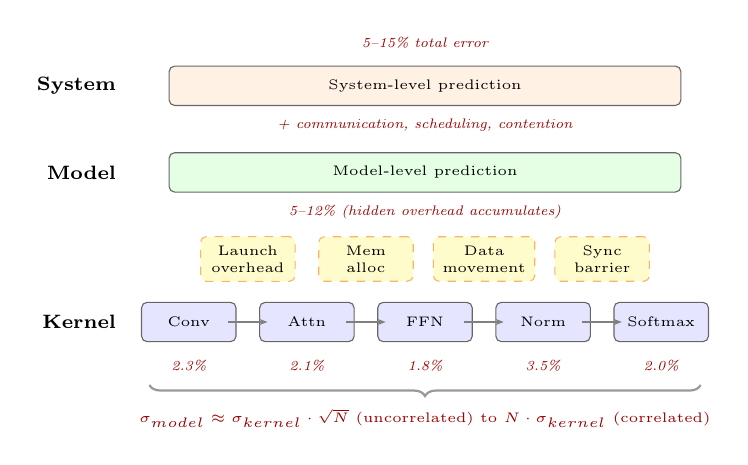
\begin{tikzpicture}[
    box/.style={draw=black!60, rounded corners=2pt, minimum width=1.2cm, minimum height=0.5cm, align=center, font=\tiny},
    err/.style={font=\tiny\itshape, text=red!60!black},
    arr/.style={-{Stealth[length=3pt]}, thick, black!50},
    brace/.style={decorate, decoration={brace, amplitude=4pt, mirror}, thick, black!40},
]

% Kernel level
\node[box, fill=blue!10] (k1) at (0,0) {Conv};
\node[box, fill=blue!10] (k2) at (1.5,0) {Attn};
\node[box, fill=blue!10] (k3) at (3,0) {FFN};
\node[box, fill=blue!10] (k4) at (4.5,0) {Norm};
\node[box, fill=blue!10] (k5) at (6,0) {Softmax};
\node[err] at (0,-0.55) {2.3\%};
\node[err] at (1.5,-0.55) {2.1\%};
\node[err] at (3,-0.55) {1.8\%};
\node[err] at (4.5,-0.55) {3.5\%};
\node[err] at (6,-0.55) {2.0\%};
\node[font=\scriptsize\bfseries, anchor=east] at (-0.8,0) {Kernel};

% Composition arrows
\draw[arr] (0.5,0) -- (1,0);
\draw[arr] (2,0) -- (2.5,0);
\draw[arr] (3.5,0) -- (4,0);
\draw[arr] (5,0) -- (5.5,0);

% Hidden errors
\node[box, fill=yellow!20, dashed, draw=orange!60] (h1) at (0.75,0.8) {Launch\\overhead};
\node[box, fill=yellow!20, dashed, draw=orange!60] (h2) at (2.25,0.8) {Mem\\alloc};
\node[box, fill=yellow!20, dashed, draw=orange!60] (h3) at (3.75,0.8) {Data\\movement};
\node[box, fill=yellow!20, dashed, draw=orange!60] (h4) at (5.25,0.8) {Sync\\barrier};

% Model level
\node[box, fill=green!10, minimum width=6.5cm] (model) at (3,1.9) {Model-level prediction};
\node[err] at (3,1.4) {5--12\% (hidden overhead accumulates)};
\node[font=\scriptsize\bfseries, anchor=east] at (-0.8,1.9) {Model};

% System level
\node[box, fill=orange!10, minimum width=6.5cm] (system) at (3,3.0) {System-level prediction};
\node[err] at (3,2.5) {+ communication, scheduling, contention};
\node[font=\scriptsize\bfseries, anchor=east] at (-0.8,3.0) {System};
\node[err] at (3,3.55) {5--15\% total error};

% Braces
\draw[brace] (-0.5,-0.8) -- (6.5,-0.8) node[midway, below=5pt, font=\tiny, text=red!60!black] {$\sigma_{\text{model}} \approx \sigma_{\text{kernel}} \cdot \sqrt{N}$ (uncorrelated) to $N \cdot \sigma_{\text{kernel}}$ (correlated)};

\end{tikzpicture}%
}
\caption{Error composition across abstraction levels. Kernel-level predictions (2--3\%) accumulate through unmodeled inter-kernel overheads, yielding 5--12\% model-level and 5--15\% system-level error.}
\label{fig:error-composition}
\end{figure}

\textbf{2. Frontier workload coverage.}
The temporal validation lag is closing for transformers but remains wide: MoE, diffusion~\cite{dynamicreasoning2026}, and dynamic inference lack validated tools; scaling laws~\cite{kaplan2020scaling,hoffmann2022chinchilla,scalinglaws2024,scalinglawguide2025} predict loss but not latency (Figure~\ref{fig:workload-coverage}).

\begin{figure}[t]
\centering
\resizebox{\columnwidth}{!}{%
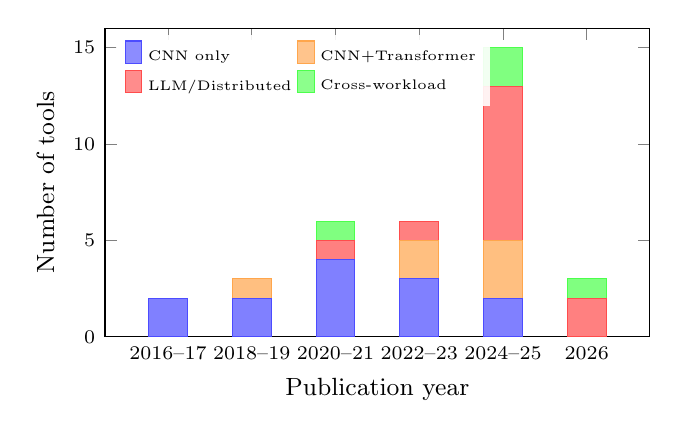
\begin{tikzpicture}
\begin{axis}[
    ybar stacked,
    bar width=14pt,
    xlabel={Publication year},
    ylabel={Number of tools},
    ymin=0, ymax=16,
    xtick={2016,2018,2020,2022,2024,2026},
    xticklabels={2016--17,2018--19,2020--21,2022--23,2024--25,2026},
    xticklabel style={font=\scriptsize},
    yticklabel style={font=\scriptsize},
    xlabel style={font=\small},
    ylabel style={font=\small},
    legend style={at={(0.02,0.98)}, anchor=north west, font=\tiny, draw=none, fill=white, fill opacity=0.9, text opacity=1, legend columns=2},
    legend cell align={left},
    height=5.5cm,
    width=8.5cm,
    enlarge x limits={abs=0.8cm},
]
\addplot[fill=blue!50, draw=blue!70] coordinates {(2016,2) (2018,2) (2020,4) (2022,3) (2024,2) (2026,0)};
\addplot[fill=orange!50, draw=orange!70] coordinates {(2016,0) (2018,1) (2020,0) (2022,2) (2024,3) (2026,0)};
\addplot[fill=red!50, draw=red!70] coordinates {(2016,0) (2018,0) (2020,1) (2022,1) (2024,8) (2026,2)};
\addplot[fill=green!50, draw=green!70] coordinates {(2016,0) (2018,0) (2020,1) (2022,0) (2024,2) (2026,1)};
\legend{CNN only, CNN+Transformer, LLM/Distributed, Cross-workload}
\end{axis}
\end{tikzpicture}%
}
\caption{Workload coverage by publication period. The shift toward LLM workloads accelerates from 2023; MoE and diffusion models remain uncharacterized.}
\label{fig:workload-coverage}
\end{figure}

\textbf{3. Hardware transfer and emerging architectures.}
Cross-family transfer (GPU$\rightarrow$TPU$\rightarrow$PIM) remains unsolved despite meta-learning (HELP) and feature-based transfer (LitePred).
PIM~\cite{upimulator2024,attacc2024,neupims2024,paise2025}, chiplets, and disaggregated designs blur memory hierarchy assumptions.

\textbf{4. Standardized evaluation infrastructure.}
No MLPerf~\cite{mlperf_training2020,mlperf_inference2020} equivalent exists for performance \emph{prediction}.
The community needs common benchmarks, shared platforms, and standardized reporting; portable formats (ONNX, Chakra~\cite{chakra2023}) and Docker-first deployment are prerequisites.

\textbf{5. Temporal stability.}
Software stack evolution (FlashAttention~\cite{flashattention2022}, CUDA updates) silently invalidates models.
nn-Meter's failure within two years demonstrates urgency; future tools should adopt continuous validation~\cite{mlperfpower2025}.

% ==============================================================================
% CONCLUSION
% ==============================================================================
\section{Conclusion}
\label{sec:conclusion}

This survey of 22 ML performance modeling tools provides accuracy-centered evaluation of five tools through independent experiments against an LLM-focused benchmark suite of 28 scenarios.
Four findings emerge.
First, \emph{self-reported accuracy is unreliable}: NeuSight's claimed 2.3\% MAPE is 5.87--27.10\% depending on GPU, while nn-Meter ($<$1\% claimed) produces no output.
Second, \emph{the five tools are complementary}---their disjoint coverage motivates a unified pipeline combining kernel prediction, communication simulation, LLM serving, and accelerator design.
Third, \emph{the composition gap dominates end-to-end error}: the 5--15\% gap between kernel and model-level prediction exceeds kernel-level error, meaning better kernel predictors have diminishing returns until composition is solved.
Fourth, \emph{50\% of modern LLM workloads lack tool support}: the fastest-growing deployment techniques---quantization, speculative decoding, LoRA, disaggregated serving---have zero coverage across all evaluated tools.
The most pressing needs are validated composition models, benchmark-driven tool development targeting uncovered LLM scenarios, and continuous accuracy validation.

%%%%%%% -- PAPER CONTENT ENDS -- %%%%%%%%

%%
%% The next two lines define the bibliography style to be used, and
%% the bibliography file.
\bibliographystyle{ACM-Reference-Format}
\bibliography{references}

\end{document}
